\chapter{Case Studies}
\label{chap:caseStudies}
This chapter illustrates aspects of the safety annex in terms of both modeling and analysis. The first section describes a large case study example called the Wheel Brake System (WBS) for an aircraft; the nominal system is modeled and extended by the safety annex. We discuss the results in terms of scalability and present the timing and minimal cut set results. An example showing the flexibility of fault modeling with the safety annex is given in the following section. The chapter concludes with a discussion on analysis timing results for a set of models. 

\section{Wheel Brake System}
\label{sec:wbs}
To demonstrate the fault modeling capabilities of the Safety Annex we will use the Wheel Brake System (WBS) described in AIR6110~\cite{AIR6110}.  This system is a well-known example that has been used as a case study for safety analysis, formal verification, and contract based design~\cite{DBLP:conf/cav/BozzanoCPJKPRT15, 10.1007/978-3-319-11936-6-7, CAV2015:BoCiGrMa, Joshi05:SafeComp}. The preliminary work for the Safety Annex was based on a simple model of the WBS~\cite{Stewart17:IMBSA}. To demonstrate a more complex fault modeling process, we constructed a functionally and structurally equivalent AADL version of the more complex WBS NuSMV/xSAP models~\cite{DBLP:conf/cav/BozzanoCPJKPRT15}.    

\begin{figure}[htbp]
	\centering
	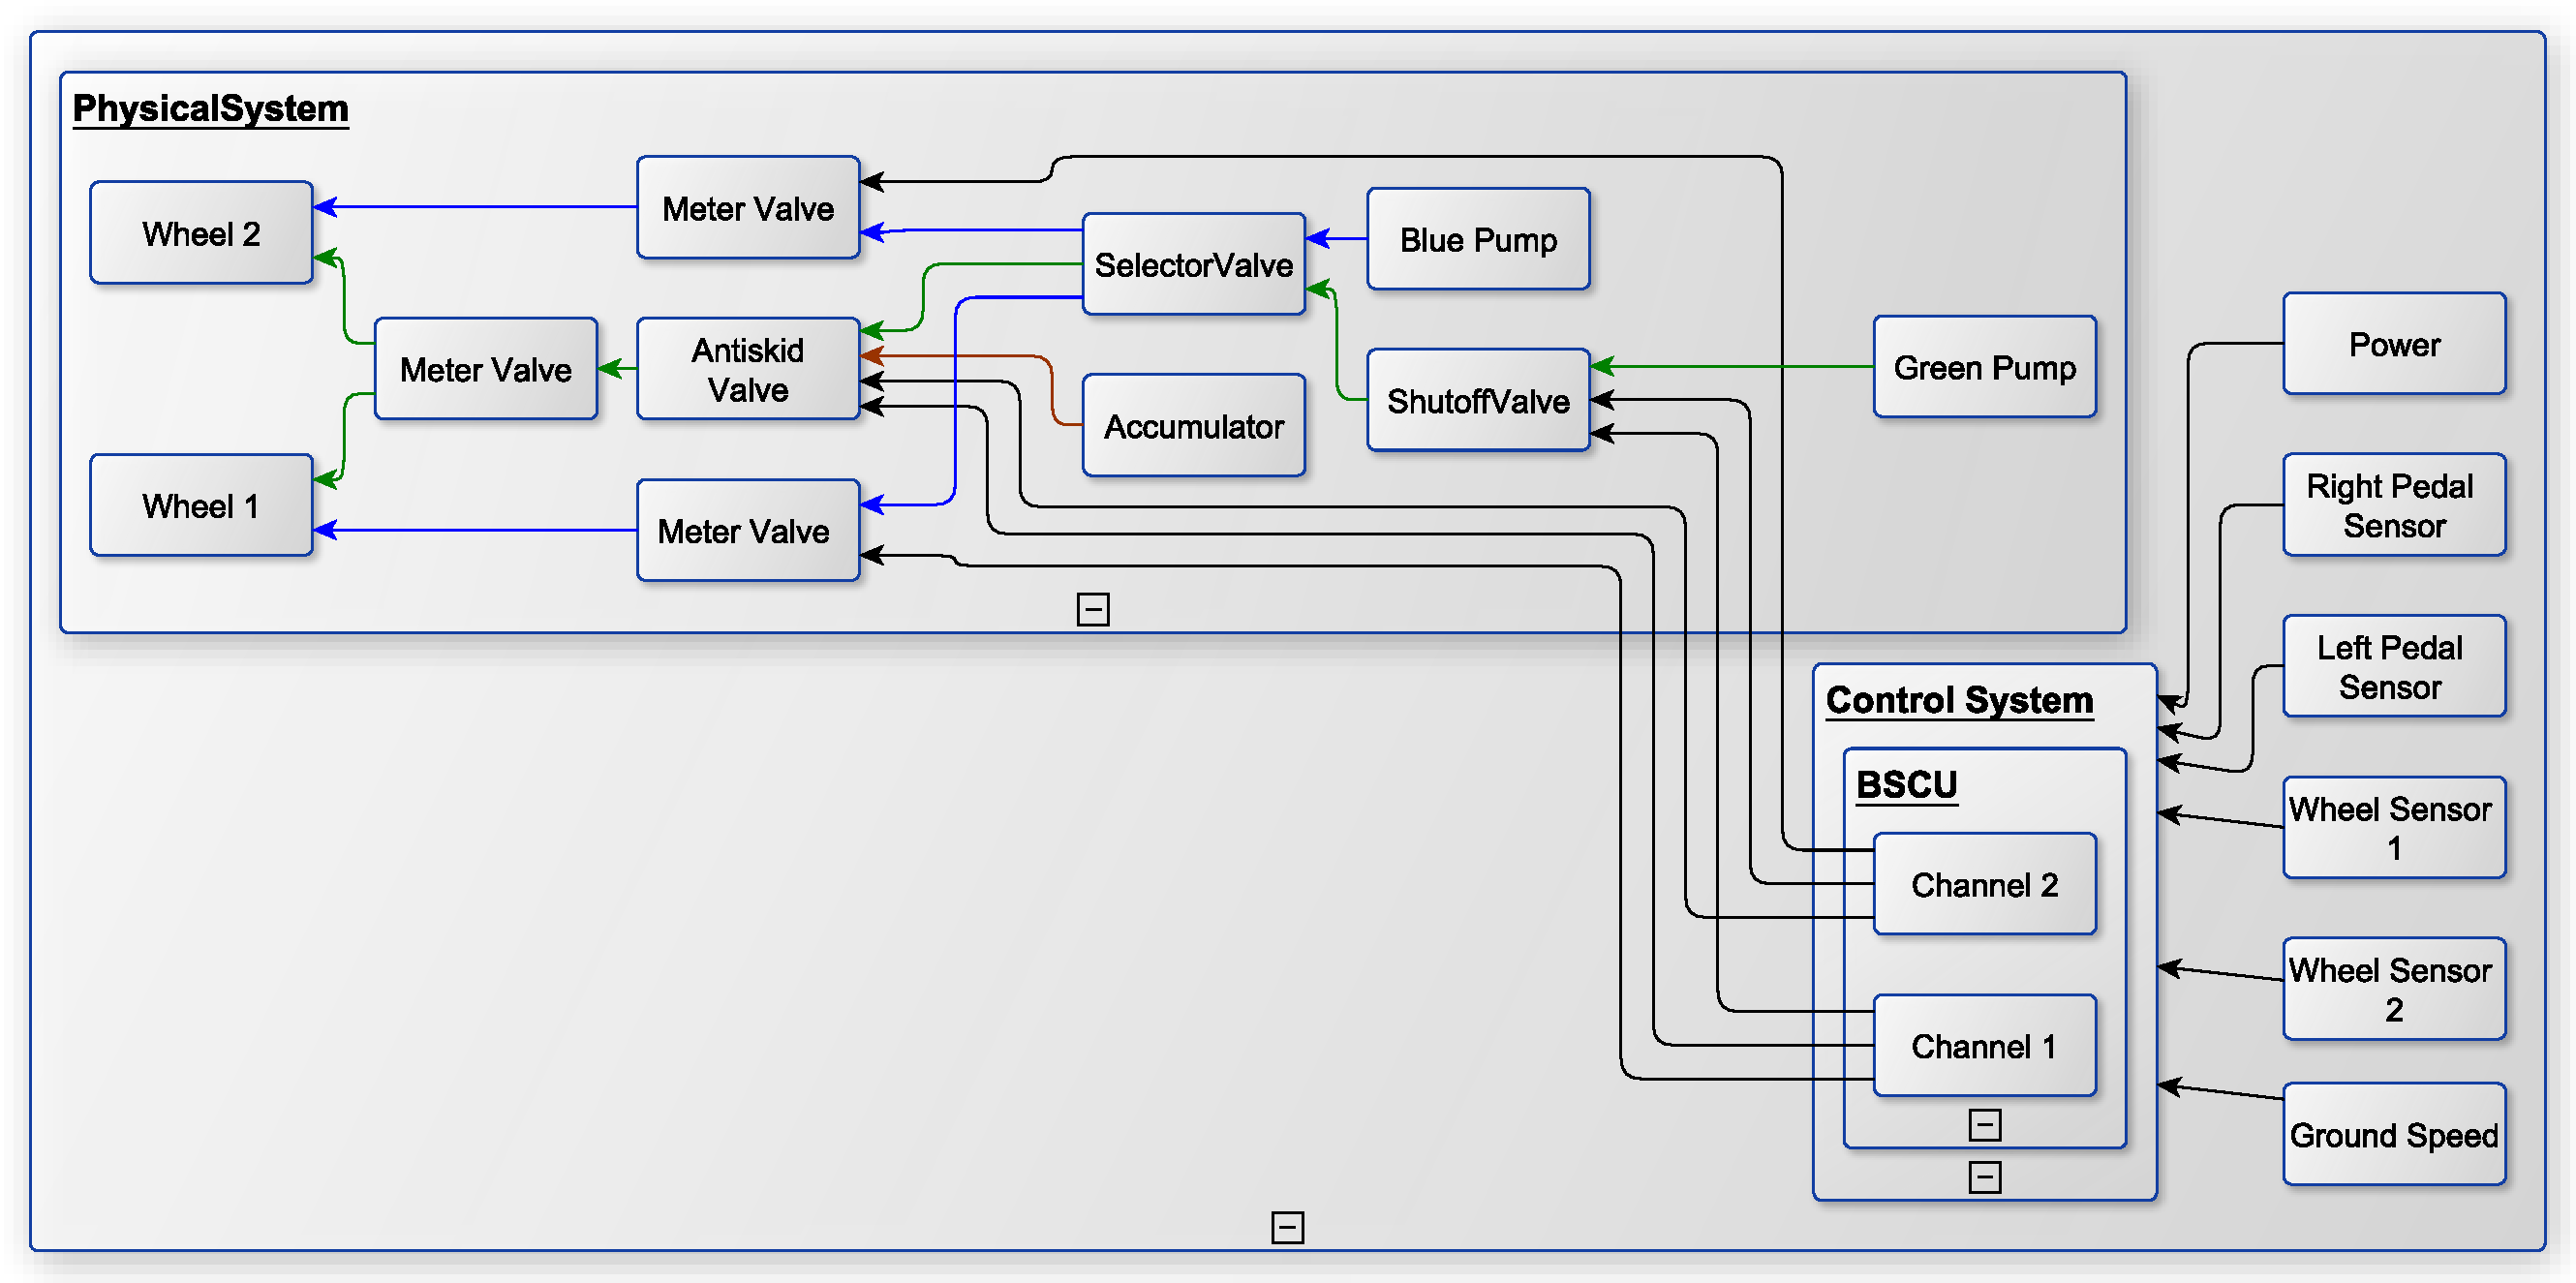
\includegraphics[trim=0 9 0 5,clip,width=\textwidth]{images/wbs_arch4_diagram.pdf}
	\caption{Simplified Two-Wheel WBS}
	\label{fig:wbs}
\end{figure} 

The WBS is composed of two main parts: the Line Replaceable Unit control system and the electro-mechanical physical system.
The control system electronically controls the physical system and contains a redundant
channel of the Braking System Control Unit (BSCU) in case a detectable fault occurs in the active channel.
 It also commands antiskid braking. % in case of skidding on the ground. 
 The physical system consists of the hydraulic circuits running from hydraulic pumps to wheel brakes as well as valves that control the hydraulic fluid flow. This system provides braking force to each of the eight wheels of the aircraft. The wheels are all mechanically braked in pairs (one pair per landing gear). For simplicity, Figure~\ref{fig:wbs} displays only two of the eight wheels. 

There are three operating modes in the WBS model:

\begin{itemize}
	\renewcommand{\labelitemi}{\textbullet}
	\item In \textit{normal} mode, the system is composed of a \textit{green} hydraulic pump and one meter valve per each of the eight wheels. Each of the meter valves are controlled through electronic commands coming from the active channel of the BSCU. These signals provide braking and antiskid commands for each wheel. The braking command is determined through a sensor on the pedal and the antiskid command is determined by the \textit{Wheel Sensors}. 
	\item In \textit{alternate} mode, the system is composed of a \textit{blue} hydraulic pump, four meter valves, and four antiskid shutoff valves, one for each landing gear. The meter valves are mechanically commanded through the pilot pedal corresponding to each landing gear. If the selector detects lack of pressure in the green circuit, it switches to the blue circuit. 
	\item In \textit{emergency} mode, the system mode is entered if the \textit{blue} hydraulic pump fails. The accumulator pump has a reserve of pressurized hydraulic fluid and will supply this to the blue circuit in emergency mode. 
\end{itemize}

The WBS architecture model in AADL contains 30 different kinds of components, 169 component instances, and a model depth of 5 hierarchical levels. 

The behavioral model is encoded using the AGREE annex and the behavior is based on descriptions found in AIR6110. The top level system properties are given by the requirements and safety objectives in AIR6110. All of the subcomponent contracts support these system safety objectives through the use of assumptions on component input and guarantees on the output. 

An example system safety property is to ensure that there is no inadvertent braking of any of the wheels. This is based on a failure condition described in AIR6110 is \textit{Inadvertent wheel braking on one wheel during takeoff shall be less than 1E-9 per takeoff}. 
Inadvertent braking means that braking force is applied at the wheel but the pilot has not pressed the brake pedal.  In addition, the inadvertent braking requires that power and hydraulic pressure are both present, the plane is not stopped, and the wheel is rolling (not skidding). The property is stated in AGREE such that inadvertent braking does \textit{not} occur, as shown in Figure \ref{fig:inadvertent_braking}. 

\begin{figure}[htbp]
	%\vspace{-0.2in}
	\begin{center}
		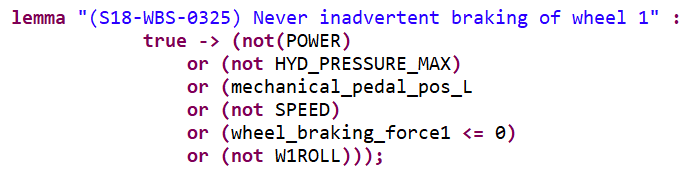
\includegraphics[width=.7\textwidth]{images/inadvertent_braking.png}
	\end{center}
	\vspace{-0.3in}
	\caption{Safety Property: Inadvertent Braking}
	\label{fig:inadvertent_braking}
	%\vspace{-0.2in}
\end{figure}

\subsection{Nominal Model Analysis}
Before performing fault analysis, users should first check that the safety properties are satisfied by the nominal design model. This analysis can be performed monolithically or compositionally in AGREE. Using monolithic analysis, the contracts at the lower levels of the architecture are flattened and used in the proof of the top level safety properties of the system. Compositional analysis, on the other hand, will perform the proof layer by layer top down, essentially breaking the larger proof into subsets of smaller problems. For a more comprehensive description of these types of proofs and analyses, see additional publications related to AGREE \cite{cofer2012compositional,QFCS15:backes} and we refer you to Section~\ref{sec:concepts}.

The WBS has a total of 13 safety properties at the top level that are supported by subcomponent assumptions and guarantees. These are shown in Table \ref{tab:safetyProperties}. Given that there are 8 wheels, contract S18-WBS-0325-wheelX is repeated 8 times, one for each wheel. The behavioral model in total consists of over 440 assumptions and guarantees after instantiation.

\begin{table}[htbp]
\begin{center}
\begin{tabular}{@{}ll}
\toprule
\textbf{S18-WBS-R-0321} \\Loss of all wheel braking during landing or RTO shall be less than $5.0 \times 10^{-7}$ per flight.                                    \\ \midrule 
\textbf{S18-WBS-R/L-0322}  \\ Asymmetrical loss of wheel braking (Left/Right) shall be less than $5.0 \times 10^{-7}$ per flight. \\ \midrule
\textbf{S18-WBS-0323} \\ Never inadvertent braking with all wheels locked shall be less than $1.0 \times 10^{-9}$ per takeoff.                                                                                                                                                                                                               \\ \midrule
\textbf{S18-WBS-0324}  \\ Never inadvertent braking with all wheels shall be less than $1.0 \times 10^{-9}$ per takeoff.                                                                                                            \\ \midrule
\textbf{S18-WBS-0325-wheelX} \\ Never inadvertent braking of wheel X shall be less than $1.0 \times 10^{-9}$ per takeoff.                                                                                                           .                                                                                                                 \\ \bottomrule
\end{tabular}
\caption{Safety Properties of the WBS}
\label{tab:safetyProperties}
\end{center} 
\end{table} 


\subsection{Fault Model Analysis}
There are two main options for fault model analysis using the Safety Annex. The first option injects faults into the Lustre program based on the restrictions placed through the fault hypothesis. The bounded model checker engine used in JKind will find counterexamples to an invalid property. These counterexamples are returned to the user and include a trace of the system state that causes the violation. This includes any active faults that were part of that violation. The second option is used to generate minimal cut sets for the model. The fault activation literals and supporting guarantees are added to the MIVC algorithm elements as described in Sections~\ref{sec:formalization} and \ref{sec:impl}, the algorithm generating the cut sets is run (Section~\ref{sec:impl}), and the results are displayed to the user. 

\subsubsection{Verification in the Presence of Faults: Max \textit{n} Analysis}
Using a max number of faults for the hypothesis, the user can constrain the number of simultaneously active faults in the model. The faults are added to the AGREE model for the verification. Given the constraint on the number of possible simultaneously active faults, the model checker attempts to prove the top level properties given these constraints. If this cannot be done, the counterexample provided will show which of the faults ($n$ or less) are active and which contracts are violated. More detail on verification of fault models can be found in Section~\ref{sec:analysisResults}. 

The WBS was verified in the presence of faults given a \texttt{max 1 fault} hypothesis using compositional analysis. The time for complete model analysis was approximately 9 minutes, but a counterexample for certain top level properties took only around 20 seconds. (Recall that when using compositional verification in the presence of faults, that hypothesis applies to each layer separately -- the results are not rolled up as in the compositional generation of minimal cut sets. The counterexample given in this analysis pertains only to faults and contracts \textit{in a given layer}, and the timing of the counterexample reflects this single layer analysis result.) 

The verification in the presence of faults with \texttt{max 1 fault} hypothesis statement provided a counterexample to the property {\em S18-WBS-0325: never inadvertent braking of wheel i}, for $i = 1, \dots 8$. This property is given in Figure~\ref{fig:inadvertent_braking}. The intuition behind the failure is that the pedal was not pressed, the sensor stated that it was pressed, braking was commanded through the digital components, and brake pressure was supplied at the wheel. This sensor fault was a single point of failure with regard to all of the inadvertent braking properties. Later in this section we look at the sensor on the pedal position in closer detail from the lens of architectural design changes led by the analysis results. 

\subsubsection{Verification in the Presence of Faults: Probabilistic Analysis} 
Given a probabilistic fault hypothesis, this corresponds to performing analysis with the combinations of faults whose occurrence probability is less than the probability threshold. This is done by inserting assertions that allow those combinations in the Lustre code. If the model checker proves that the safety properties can be violated with any of those combinations, one of such combination will be shown in the counterexample. Probabilistic analysis done in this way must utilize the monolithic AGREE option. 

Recall that when using the \texttt{max 1 fault} hypothesis statement on the WBS, we found that the sensor was a single point of failure for multiple properties. The probability of this particular sensor failing is given in AIR6110~\cite{AIR6110} as $1.0 \times 10^{-2}$. The probabilistic hypothesis was set according to the thresholds given per property (see Table~\ref{tab:safetyProperties}) and the analysis was run monolithically on the WBS model. The total time {\em to generate a counterexample} for violated properties using a probabilistic hypothesis with monolithic analysis varied depending on the safety property; the range of times was between 15 seconds and 9 minutes. The property that took the longest to generate a counterexample for was {\em S18-WBS-0323: never inadvertent braking with all wheels locked shall be less than $1.0 \times 10^{-9}$ per takeoff.} The formula for this property references all 8 wheels and numerous subcomponents, most of which have faults associated with them. The low probability threshold combined with the formula complexity and the exponential increase in fault combinations likely served to make this the longest time in counterexample generation. For a full discussion on use of probabilistic thresholds in compositional analysis, see Section~\ref{sec:prob_generate}.

\subsubsection{Generate Minimal Cut Sets: Max \textit{n} Analysis}
\label{sec:maxN_generate}
As described in Section~\ref{sec:impl}, we use the \aivcalg algorithm to provide a full enumeration of all minimal set of model elements necessary for the proof of each top-level safety property in the model, and then transform all MIVCs into all minimal cut sets. In max $n$ analysis, the minimal cut sets are pruned to include only those with at cardinality less than or equal to the number $n$ specified in the fault hypothesis.

Generate minimal cut set analysis was performed on the Wheel Brake System and results are shown in Table~\ref{tab:wbs_maxN_results}. Notice in Table~\ref{tab:wbs_maxN_results}, the label across the top row refers to the cardinality (\textit{n}) and the corresponding column shows how many cut sets are generated of that cardinality. When the analysis is run, the user specifies the value \textit{n}. This gives cut sets of cardinality less than or equal to \textit{n}. Table~\ref{tab:wbs_maxN_results} shows the total number of cut sets of cardinality \textit{n}. The total number of cut sets computed at the given threshold is the sum across a row. (For the full text of the properties, see Table~\ref{tab:safetyProperties}.) 


\begin{table}[htbp]
\begin{center}
    \begin{tabular}{ | l | l | l | l | l | l |}
    \hline
    \textbf{Property} & $\bm{n = 1}$ & $\bm{n = 2}$ & $\bm{n = 3}$ & $\bm{n = 4}$ 
		& $\bm{n = 5}$    \\ \hline \hline
    0321 & 7 & 0 & 0 & 256 & 57,600   \\ \hline
    0322-R & 75 & 0 & 0 & 0 & 0  \\ \hline
    0322-L & 75 & 0 & 0 & 0 & 0  \\ \hline
    0323 & 182 & 0 & 0 & 0 & 0  \\ \hline
    0324 & 8 & 3,665 & 28,694 & 883,981 & - \\ \hline
    0325-WX & 33 & 0 & 0 &0 &0 \\ \hline
    \end{tabular}
    \caption{WBS Minimal Cut Set Results for Max \textit{n} Hypothesis}
    \label{tab:wbs_maxN_results}
    \end{center}
\end{table}


As can be seen in Table~\ref{tab:wbs_maxN_results}, the number of cut sets increases proportional to the cardinality of the cut sets. Intuitively, this can be understood as simple combinations of faults that can violate the hazard; if more things go wrong in a system at the same time, the more likely a property will be violated. Property S18-WBS-0324 with a max fault hypothesis of 5 was unable to finish due to an out of memory error. At the time that the error was thrown, the number of cut sets exceeded 1.5 million. In practice, it is not likely that an analyst will manually sift through a million or more cut sets, but rather will filter out the combinations that are sufficiently unlikely to occur. A probabilistic approach would be warranted in these situations. 

The next analysis shows the difference between the time it takes to generate all MIVCs and the time it takes to transform those MIVCs into minimal cut sets. Each column of Table~\ref{tab:wbs_mincut} labeled with the value of \textit{n} gives the fault hypothesis threshold for that analysis run. For comparison with the number of minimal cut sets generated per property, we refer to Table~\ref{tab:wbs_maxN_results}\footnote{The property S18-WBS-0325-WX is symmetric for all eight wheels. For readability, we only include wheel one verification timing results in Table~\ref{tab:wbs_mincut}. Likewise for property 0322-L/R.}.
\begin{table}[htbp]
\begin{center}
    \begin{tabular}{ | l | l | l | l | l | l | l |}
    \hline
    \textbf{Property} &  MIVC Gen & $n=1$ & $n=2$ & $n=3$ & $n=4$ & $n=5$     \\ \hline \hline
    0321 & 396.417 & 5.913 & 5.468 & 5.61 & 5.636 & 11.925  \\ \hline
    0322-L  & 407.078 & 5.931 & 5.435 & 5.302 & 5.268 & 5.243 \\ \hline
    0323 & 412.926 & 6.397 & 6.452 & 6.420  & 5.309 & 5.459\\ \hline
    0324 & 446.610 & 41.334 & 41.744 & 44.062 & 69.142 & -\\ \hline
    0325-W1 & 391.137 & 5.632 & 5.388 &5.359 &5.301 & 5.236 \\ \hline
    \end{tabular}
    \caption{WBS Analysis Time in Seconds}
    \label{tab:wbs_mincut}
    \end{center}
\end{table}
The overall time of the algorithms used for minimal cut set generation is quite small compared to the nominal analysis and extended model analysis time. This is not altogether surprising; the nominal and extended analysis is contending with an infinite state model checking problem whereas the algorithms presented to generate minimal cut sets deal with set element algorithms and boolean formula manipulation. The greatest time recorded was for property S18-WBS-0324 at $n = 4$; the reason is clear when comparing this with Table~\ref{tab:wbs_maxN_results}: the total number of minimal cut sets computed for this threshold is 916,349.  

\subsubsection{Generate Minimal Cut Sets: Probabilistic Analysis}
\label{sec:prob_generate}
Both probabilistic analysis and max $n$ analysis use the same underlying minimal cut set generation algorithm, but in probabilistic analysis the minimal cut sets are pruned to include only those fault combinations whose probability of simultaneous occurrence exceed the given threshold in the hypothesis. 

The probabilistic analysis for the WBS was given a top level threshold per property as stated in AIR6110 and shown in Table~\ref{tab:safetyProperties}. The faults associated with various components were all given probability of occurrence according to the AIR6110 document~\cite{AIR6110}. The table shows the property name and associated probability. The generation of minimal cut sets provided all sets that violate that property whose combined probabilities (assuming independence) are greater than the threshold. The number of sets per cardinality are listed in the table. 

\begin{table}[htbp]
\begin{center}
    \begin{tabular}{ | l | l | l | l | l | l | l | }
    \hline
    \textbf{Property} & $n=1$ & $n=2$ & $n=3$ & $n=4$ 
		& $n=5$    \\ \hline \hline
    0321: $5.0 \times 10^{-7}$ & 7 & 0 & 0 & 256 & 0   \\ \hline
    0322-R: $5.0 \times 10^{-7}$ & 75 & 0 & 0 &0 &0   \\ \hline
    0322-L: $5.0 \times 10^{-7}$ & 75 & 0 & 0 & 0 & 0    \\ \hline
    0323: $1.0 \times 10^{-9}$ & 182 & 0 & 0 & 0 & 0    \\ \hline
    0324: $1.0 \times 10^{-9}$ & 8 & 3665 & 0 & 0 & 0   \\ \hline
    0325-W1: $1.0 \times 10^{-9}$ & 33 & 0 & 0 &0 &0    \\ \hline
    \end{tabular}
    \caption{WBS Minimal Cut Set Results for Probabilistic Hypotheses}
    \label{tab:wbs_prob_results}
    \end{center}
\end{table}

As shown in Table~\ref{tab:wbs_prob_results}, the number of allowable combinations drops considerably when given probabilistic threshold as compared to just fault combinations of certain cardinalities. For example, one contract (inadvertent wheel braking of all wheels) had over a million minimal cut sets produced when looking at it in terms of max N analysis, but after taking probabilities into account, it is seen on Table~\ref{tab:wbs_prob_results} that the likely contributors to a hazard are minimal cut sets of cardinality one. The probabilistic analysis eliminated many thousands of cut sets from consideration. The total computation time for these runs is given in Table~\ref{tab:analysisTimeWBSProb}.


\begin{table}[htbp]
\begin{center}
    \begin{tabular}{ | l | l | l | l | l | l | l | }
    \hline
    \textbf{Property} & Total Analysis Time   \\ \hline \hline
    R-0321: $5.0 \times 10^{-7}$ & 433.144 sec  \\ \hline
    R-0322: $5.0 \times 10^{-7}$  & 431.954 sec  \\ \hline
    L-0322: $5.0 \times 10^{-7}$  & 429.081 sec    \\ \hline
    0323: $1.0 \times 10^{-9}$  & 571.216 sec    \\ \hline
    0324: $1.0 \times 10^{-9}$ & 589.07 sec   \\ \hline
    0325-W1: $1.0 \times 10^{-9}$ & 430.021 sec    \\ \hline
    \end{tabular}
    \caption{WBS Minimal Cut Set Time for Probabilistic Hypothesis}
    \label{tab:analysisTimeWBSProb}
    \end{center}
\end{table}


It is clear that the lower probabilistic threshold for properties 0323-0325-WX allowed more fault combinations to be possible which increased computation time. One must also recall property 0324 from the max \textit{n} analysis whose threshold of $n=4$ produced close to a million cut sets of various cardinalities. The pruning according to probabilities cut out many of these sets from consideration; they are sufficiently unlikely to occur together. 

\subsubsection{Display Results from Generate Minimal Cut Sets}
Results from Generate Minimal Cut Sets analysis can be represented in one of the following forms. 
\begin{enumerate}
\item The minimal cut sets can be presented in text form with the total number per property, cardinality of each, and description strings showing the property and fault information. A sample of this output is shown in Figure~\ref{fig:detailedMCS}. 
\begin{figure}[htbp]
	\hspace*{-2cm}
	\vspace{-0.1in} 
	\begin{center}
		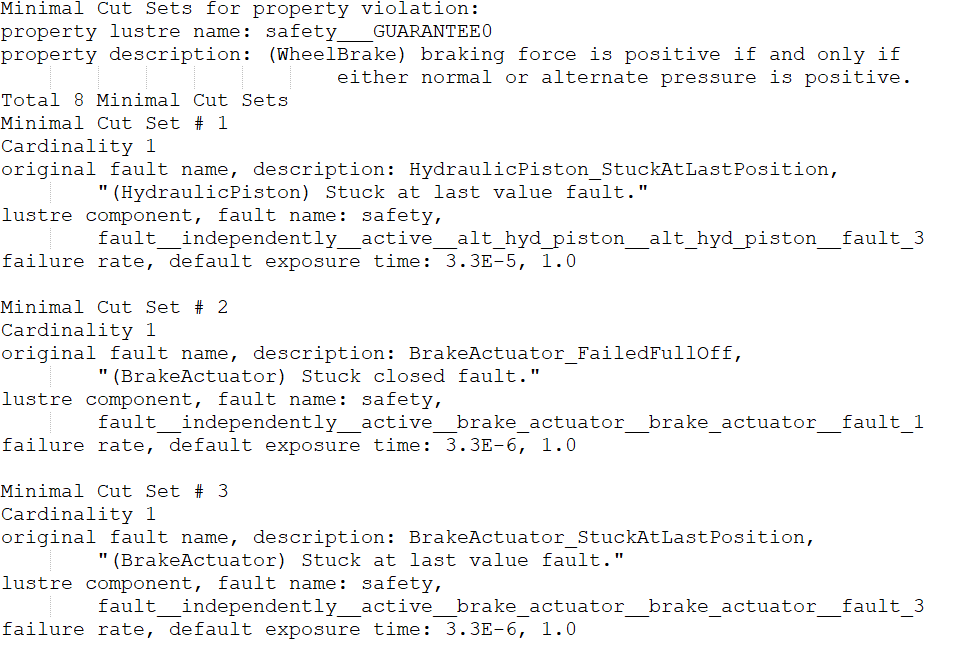
\includegraphics[scale=0.7]{images/wbsMCSDesc.png}
	\caption{Detailed Output of Minimal Cut Sets}
		\label{fig:detailedMCS}
	\end{center}
\end{figure}

\item The minimal cut set information can be presented in tally form. This does not contain the fault information in detail, but instead gives only the tally of cut sets per property. This is useful in large models with many cut sets as it reduces the size of the text file. An example of this output type is seen in Figure~\ref{fig:tallyMCS}.
\begin{figure}[htbp]
	\hspace*{-2cm}
	\vspace{-0.1in} 
	\begin{center}
		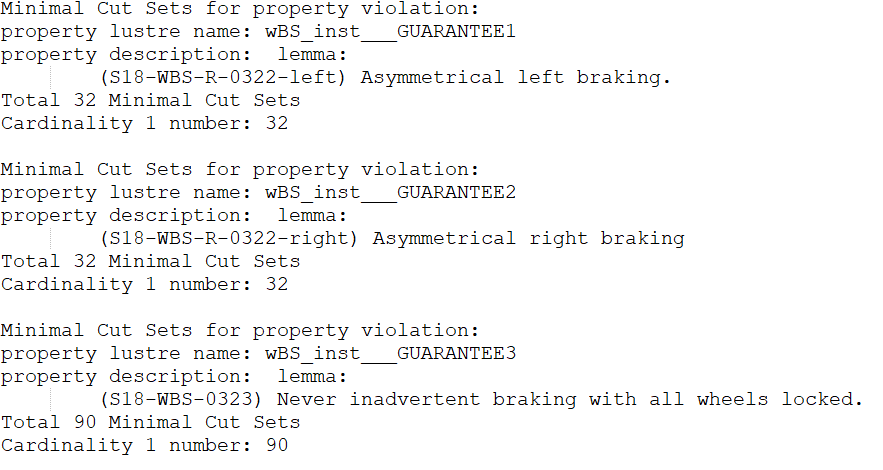
\includegraphics[scale=0.7]{images/wbsMCSTally.png}
	\caption{Tally Output of Minimal Cut Sets}
		\label{fig:tallyMCS}
	\end{center}
\end{figure}

\end{enumerate}

\subsubsection{Use of Analysis Results to Drive Design Change}
\label{sec:designChange}
We use a single top level requirement of the WBS: {\em S18-WBS-0323: Never inadvertent braking with all wheels locked} to illustrate how Safety Annex can be used to detect design flaws and how faults can affect the behavior of the system. 

Upon running max $n$ compositional fault analysis with $n = 1$, a pedal sensor fault was shown to be a single point of failure for the inadvertent braking properties. 
\begin{figure}[htbp]
	%\vspace{-0.2in}
	\begin{center}
		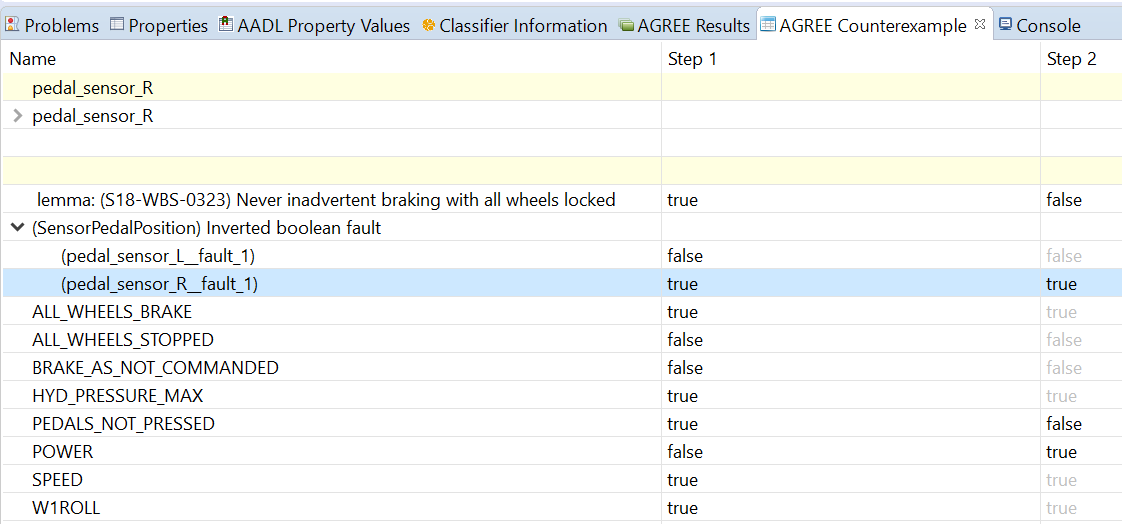
\includegraphics[width=0.8\textwidth]{images/counterexample.png}
	\end{center}
	\vspace{-0.3in}
	\caption{Counterexample for Inadvertent Braking}
	\label{fig:counterexample}
	%\vspace{-0.2in}
\end{figure} 
A counterexample is shown in Figure \ref{fig:counterexample} showing the active fault on the pedal sensor. Depending on the goals of the system, the architecture currently modeled, and the mitigation strategies that are desired, various strategies are possible to mitigate the problem.

\begin{itemize}
\item Possible mitigation strategy 1: Monitor system can be added for the sensor: A monitor sub-component can be modeled in which it accesses the mechanical pedal as well as the signal from the sensor. If the monitor finds discrepancies between these values, it can send an indication of invalid sensor value to the top level of the system. In terms of the modeling, this would require a change to the behavioral contracts which use the sensor value. This validity would be taken into account through the means of $valid \land pedal\_sensor\_value$. 
%In the real system however, this mitigation would need to be taken into account. Whether this is a flag to the pilot who can then override the electrical system and switch to a different mode or perform some other action to mitigate the failed sensor must be discussed and implemented. 

\item Possible mitigation strategy 2: Redundancy can be added to the sensor: A sensor subsystem can be modeled which contains 3 or more sensors. The overall output from the sensor system may utilize a voting scheme to determine validity of sensor reading. There are multiple voting schemes that are possible, one of which is a majority voting (e.g. one sensor fails, the other two take majority vote and the correct value is passed). 
When three sensors are present, this mitigates the single point of failure problem. New behavioral contracts are added to the sensor system to model the behavior of redundancy and voting. 
\end{itemize}
\begin{figure}[htbp]
	%\vspace{-0.2in}
	\begin{center}
		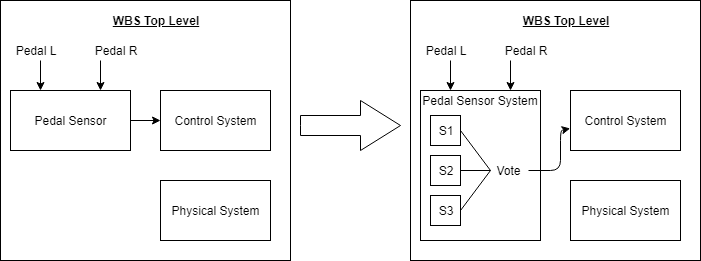
\includegraphics[width=0.7\textwidth]{images/sensorsystem.png}
	\end{center}
	\vspace{-0.3in}
	\caption{Architectural Changes for Fault Mitigation}
	\label{fig:sensorsystem}
	%\vspace{-0.2in}
\end{figure}
In the case of the pedal sensor in the WBS, the latter of the two strategies outlined above was implemented. A sensor system was added to the model which held three pedal sensors. The output of this subsystem was constrained using a majority voting scheme. Upon subsequent runs of the analysis (regardless which type of run was used), resilience was confirmed in the system regarding the failure of a single pedal sensor. Figure \ref{fig:sensorsystem} outlines the architectural changes that were made in the model.

As can be seen through this single example, a system as large as the WBS would benefit from many iterations of this process. Furthermore, if the model is changed even slightly on the system development side, it would automatically be seen from the safety analysis perspective and any negative outcomes would be shown upon subsequent analysis runs. This effectively eliminates any miscommunications between the system development and analysis teams and creates a new safeguard regarding model changes. 

For more information on types of fault models that can be created as well as details on analysis results, see the users guide located in the GitHub repository \cite{SAGithub}. This repository also contains all models used in this project. 
\section{Process ID Example}
\label{sec:pid}
The illustration of asymmetric fault implementation can be seen through a simple example where 4 nodes report to each other their own process ID (PID). Each node has a 1-3 connection and thus each node is a candidate for an asymmetric fault. Given this architecture, a top level contract of the system is simply that all nodes report and see the correct PID of all other nodes. Naturally in the absence of faults, this holds. But when one asymmetric fault is introduced on any of the nodes, this contract cannot be verified. What is desired is a protocol in which all nodes agree on a value (correct or arbitrary) for all PIDs. 

\subsection{The Agreement Protocol Behavioral Implementation}
In order to mitigate this problem, special attention must be given to the behavioral model. Using the strategies outlined in previous research~\cite{bracha1987asynchronous,Driscoll-Byzantine-Fault}, the agreement protocol is specified in AGREE to create a model resilient to one active Byzantine fault. 

The objective of the agreement protocol is for all correct (non-failed) nodes to eventually reach agreement on the PID values of the other nodes. There are $n$ nodes, possibly $f$ failed nodes. The protocol requires $n > 3f$ nodes to handle a single fault. The point is to achieve distributed agreement and coordinated decisions.
The properties that must be verified in order to prove the protocol works as desired are as follows: 
\begin{itemize}
	\item All correct (non-failed) nodes eventually reach a decision regarding the value they have been given.  In this solution, nodes will agree in $f+1$ time steps or rounds of communication.   
	\item If the source node is correct, all other correct nodes agree on the value that was originally sent by the source.  
	\item If the source node is failed, all other nodes must agree on some predetermined default value.  
\end{itemize}

The updated architecture of the PID example is shown in Figure~\ref{fig:PIDArch}. 
\begin{figure}[!htb]
        \center{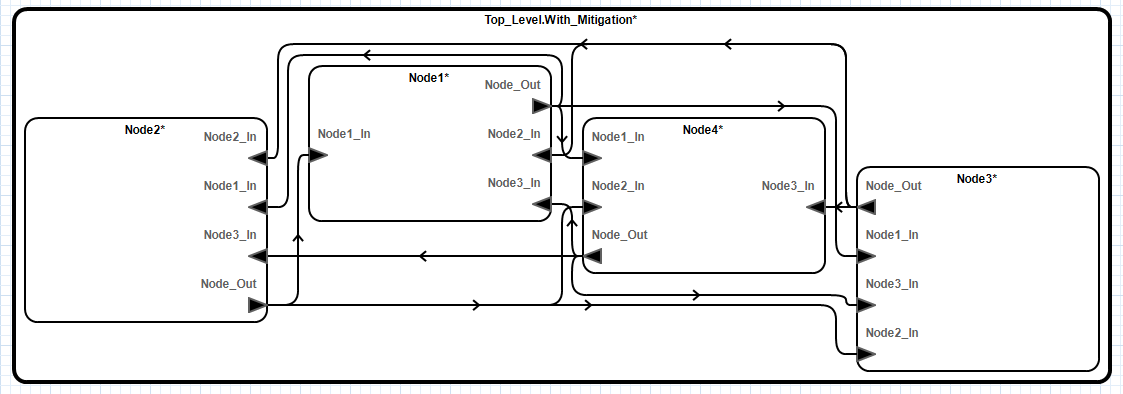
\includegraphics[width=\textwidth] {images/PIDArch.png}}
        \caption{\label{fig:PIDArch} Updated PID Example Architecture}
\end{figure}

Each node reports its own PID to all other nodes in the first round of communication. In the second round, each node informs the others what they saw in terms of %everyones
everyone's PIDs. %Thus, new connections are added for this second round of communication.
The outputs from a node are described in Figure~\ref{fig:NodeOutputsPID}. %\janet{The figure needs to be updated, as node 2 sends to node 1, 2, 3; and node 3 sends to node 1, 2, 4; and node 4 sends to node 1, 2, 3}
\begin{figure}[!htb]
        \center{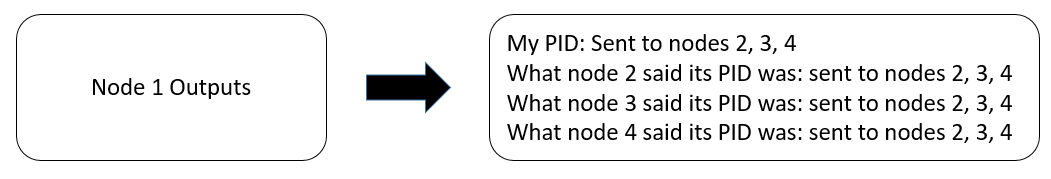
\includegraphics[width=0.9\textwidth] {images/NodeOutputsPID.png}}
        \caption{\label{fig:NodeOutputsPID} Description of the Outputs of Each Node in the PID Example}
\end{figure}
%These new connections 
These outputs are modeled as a nested data implementation in AADL and each field corresponds to a PID from a node. The AADL code fragment defining this data implementation is shown in Figure~\ref{fig:PIDNodeData}.

\begin{figure}[!htb]
        \center{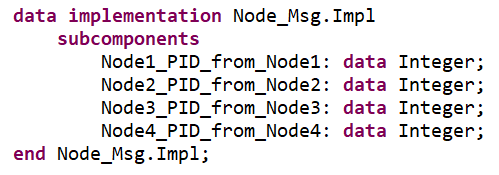
\includegraphics[width=0.7\textwidth] {images/PIDNodeData.png}}
        \caption{\label{fig:PIDNodeData} Data Implementation in AADL for Node Outputs}
\end{figure}

The fault definition for %that is inserted explicitly into the model is connected to 
each node's output and can effect the data fields arbitrarily. This is a nondeterministic fault in two ways. It is nondeterministic how many receiving nodes see incorrect values and it is nondeterministic how many of the data fields are affected by this fault. This can be accomplished through the fault definition shown in Figure~\ref{fig:PIDFaultNode} and the fault node definition in Figure~\ref{fig:PIDFaultDef}. 

\begin{figure}[!htb]
        \center{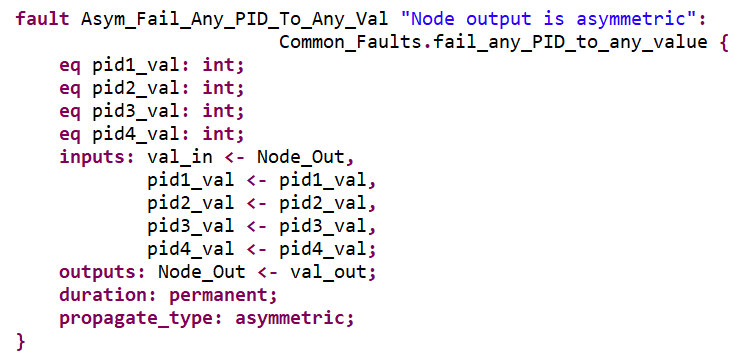
\includegraphics[width=0.9\textwidth] {images/PIDFaultNode.png}}
        \caption{\label{fig:PIDFaultNode} Fault Definition on Node Outputs for PID Example}
\end{figure}

\begin{figure}[!htb]
        \center{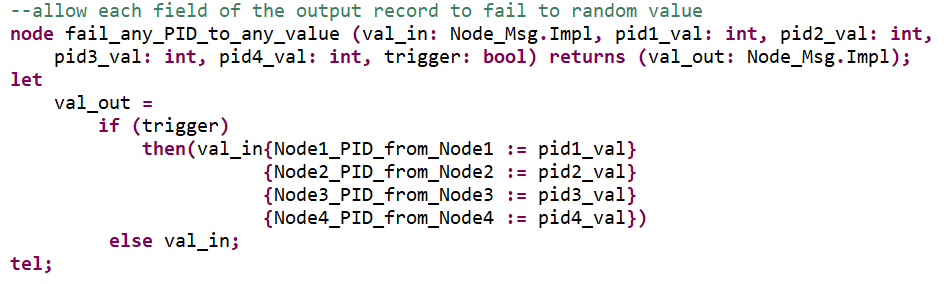
\includegraphics[width=0.9\textwidth] {images/PIDFaultDef.png}}
        \caption{\label{fig:PIDFaultDef} Fault Node Definition for PID Example}
\end{figure}

Once the fault model is in place, the implementation in AGREE of the agreement protocol is developed. As stated previously, there are two cases that must be considered in the contracts of this system. 
\begin{itemize}
	\item In the case of no active faults, all nodes must agree on the correct PID of all other nodes. 
	\item In the case of an active fault on a node, all non-failed nodes must agree on a PID for all other nodes. 
\end{itemize}

These requirements are encoded in AGREE through the use of the following contracts. Figure~\ref{fig:PIDContract1} and Figure~\ref{fig:PIDContract2} show example contracts regarding Node 1 PID. There are similar contracts for each node's PID. 
\begin{figure}[!htb]
        \center{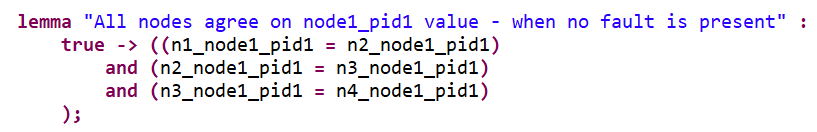
\includegraphics[width=0.9\textwidth] {images/PIDContract1.png}}
        \caption{\label{fig:PIDContract1} Agreement Protocol Contract in AGREE for No Active Faults}
\end{figure}

\begin{figure}[!htb]
        \center{\includegraphics[width=0.9\textwidth] {images/PIDCOntract2.png}}
        \caption{\label{fig:PIDContract2} Agreement Protocol Contract in AGREE Regarding Non-failed Nodes}
\end{figure}


\textbf{Referencing Fault Activation Status}
To fully implement the agreement protocol, it must be possible to describe whether or not a component has failed; this is performed through the use of a \textit{fault activation statement}. The user first defines \textit{eq} variables in AGREE that will correspond to specific faults in components. Each of the \textit{eq} variables declared in AGREE (i.e., \textit{n1\_failed, n2\_failed, n3\_failed, n4\_failed}) is linked to the fault activation status of the \textit{Asym\_Fail\_Any\_PID\_To\_Any\_Value} fault defined in a node subcomponent instance of the %top level 
AADL system implementation (i.e., \textit{node1}, \textit{node2}, \textit{node3}, \textit{node4}). The fault activation statements for the PID example are shown in Figure~\ref{fig:PID_faultActivationStmt}.

\begin{figure}[!htb]
        \center{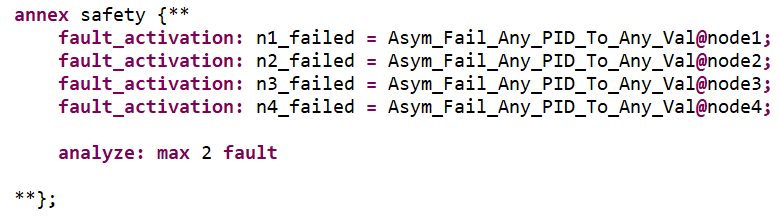
\includegraphics[width=0.9\textwidth] {images/PID_faultActivationStmt.png}}
        \caption{\label{fig:PID_faultActivationStmt} Fault Activation Statement in PID Example}
\end{figure}

\subsection{Nominal and Fault Model Analysis}
The nominal model verification shows that all properties are valid. Upon running verification in the presence of faults with maximum one active fault, the first four properties stating that all nodes agree on the correct value (Figure~\ref{fig:PIDContract1}) fail. This is expected since this property is specific to the case when no faults are present in the model. The remaining 4 top level properties (Figure~\ref{fig:PIDContract2}) state that all non-failed nodes reach agreement in two rounds of communication. These are verified valid when any one asymmetric fault is present. This shows that the agreement protocol was successful in eliminating a single point of asymmetric failure from the model. Furthermore, when changing the number of allowed faults to two, these properties do not hold. This is expected given the theoretical result that $3f+1$ nodes are required in order to be resilient to $f$ faults and that $f+1$ rounds of communication are needed for successful protocol implementation.

A summary of the results follows. 
\begin{itemize}
	\item Nominal model: All top level guarantees are verified. All nodes output the correct value and all agree. 
	\item Fault model with one active fault: The first four guarantees fail (when no fault is present, all nodes agree: shown in Figure~\ref{fig:PIDContract1}). This is expected if faults are present. The last four guarantees (all non-failed nodes agree) are verified as true with one active fault. 
	\item Fault model with two active faults: All 8 guarantees fail. This is expected since in order to be resilient up to two active faults ($f=2$), we would need $3f + 1 = 7$ nodes and $f+1 = 3$ rounds of communication. 
\end{itemize}

This example illustrates the correct handling of such faults and how to utilize the capabilities of the safety annex to model asymmetric failures and test that a system is resilient to such faults. 


\section{Discussion on Timing Results}
\label{sec:timing}
Given that the safety annex has been developed within the course of this research, there was no pre-existing benchmark models with which to conduct experiments and collect data for comparison with existing tools. As described in Section~\ref{sec:modelCheckingInSA}, there are a few related research tools that perform similar analyses, e.g., xSAP~\cite{DBLP:conf/tacas/BittnerBCCGGMMZ16}, AltaRica~\cite{signoret1998altarica}, SAML~\cite{Gudemann:2010:FQQ:1909626.1909813}, but all of these perform analysis over different modeling languages, use varying analysis methodology, and some even separate fault models from the system modeling language.

Throughout the course of this research, a small number of system models have been developed that illustrate various aspects of modeling and analysis capabilities. These range in size from quite simple two component single layer systems up to the large WBS example outlined in Section~\ref{sec:wbs}. But notice that the size of the model in terms of the architecture does not completely capture the analysis timing results. For example, a single layer architecture containing two components is small in terms of AADL models, but the nominal AGREE model may contain numerous assumptions and guarantees, and likewise a large number of faults, both of which increase computation time for proofs and for minimal cut set generation compared to a small architectural model with fewer contracts and faults. Likewise, the total number of contracts do not tell the whole story; that number does not give insight into the complexity of the formulas in the contracts. When discussing results of the fault model analysis, one must not only take into account the number of faults defined in a model, but also the probabilistic threshold, possible fault combinations that are allowed to be active at once, and the complexity of the contracts within the model. Given all of this, it is not so straightforward to run a single analysis and make comparisons along these axes, so we provide enough comparison to glean interesting information regarding the feasibility of the approach. All following analyses were run on an Intel Core i7 with a 2.80GHz CPU and 16 GB RAM. 

\paragraph{Nominal Model:} As a baseline to the analysis comparisons we provide, we run compositional nominal analysis on the 18 AADL models extended with AGREE contracts. The analysis includes property verification and component consistency checks; this is the analysis that any user would run on a nominal model with no interwoven faults. 

\paragraph{Extended model, no faults active:} Since a safety analyst extends the nominal model with fault definitions and constraints, we want to see the results of that extension in terms of additional verification time. The model grows in size with each fault that is defined in multiple ways. There is a node definition in the Lustre model corresponding to the fault behavior, there are five variables for each fault added to the model, and each of those variables has constraints written in Lustre. There are also constraints on the new fault related variables that correspond to the fault hypothesis statement. We wish to see how these extensions increases verification time when no faults are active within the model; this will give insight into the feasibility of verifying the extension alone and how costly that extension may be. 

\paragraph{Extended model, one fault active:} The reason we wish to activate a single fault in the model is to see how removing the constraint that {\em no} faults are active (as in the extended case above) changes the analysis time. By giving a single active fault constraint, the model checker is required to determine which of the faults may violate a property and thus must iterate through the fault possibilities. If one or more of those faults violate a property, a counterexample is generated which may also add to fault model verification time. 

To this end, we performed the above three types of analysis on the 18 models and graphed the results together as shown in Figure~\ref{fig:graphComp15Models}. 

\begin{figure}[htbp]
	%\vspace{-0.2in}
	\begin{center}
		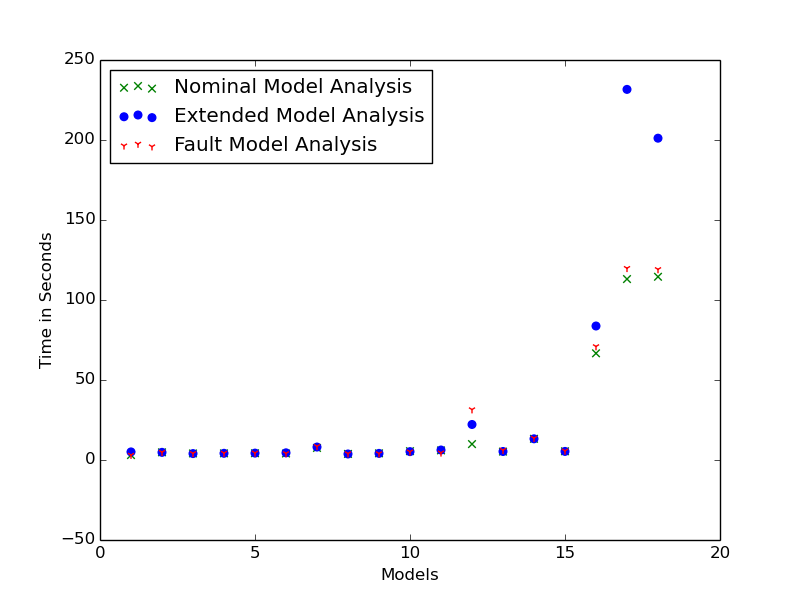
\includegraphics[width=.7\textwidth]{images/graphComp15Models.png}
	\end{center}
	\vspace{-0.3in}
	\caption{Nominal, Extended, and One Fault Verification on 18 Models}
	\label{fig:graphComp15Models}
	%\vspace{-0.2in}
\end{figure}

The first 15 models are similar in architectural and contractual size and the time differences between the three forms of analysis are negligible. Model 12 shows a greater irregularity between the nominal, extended, and fault analysis times and this is most likely due to the complexity of both the faults and contracts in the model. Models 16-18 show the greatest differences in timing results and are the largest of the set. Interestingly enough, the extended model analysis time was far greater than both the nominal and fault model analysis time. The reason for this may be due to a greater number of model elements in the extended model compared with the amount of time needed to find a counterexample. 

\paragraph{Extended model, probabilistic threshold:} In the implementation of the safety annex, a preprocessing step to probabilistic analysis is to compute all possible combinations of faults whose probability exceeds the threshold. This is inserted into the Lustre model as an assertion that states only these combinations can be active at once. If there is such a combination that violates a property, it will be shown. Compositional probabilistic analysis can only be performed through the generation of minimal cut sets; therefore, this analysis was first performed using a monolithic probabilistic approach and then a compositional minimal cut set approach to show the comparison. To illustrate how the probabilistic threshold changes analysis results and timing, we perform this analysis on a larger model: the wheel brake system with 4 wheels. This is a pared down version of what was described in Section~\ref{sec:wbs}, but still contains over 250 contracts among 66 components with faults defined for all leaf level components of the system. 

\begin{figure}[htbp]
	%\vspace{-0.2in}
	\begin{center}
		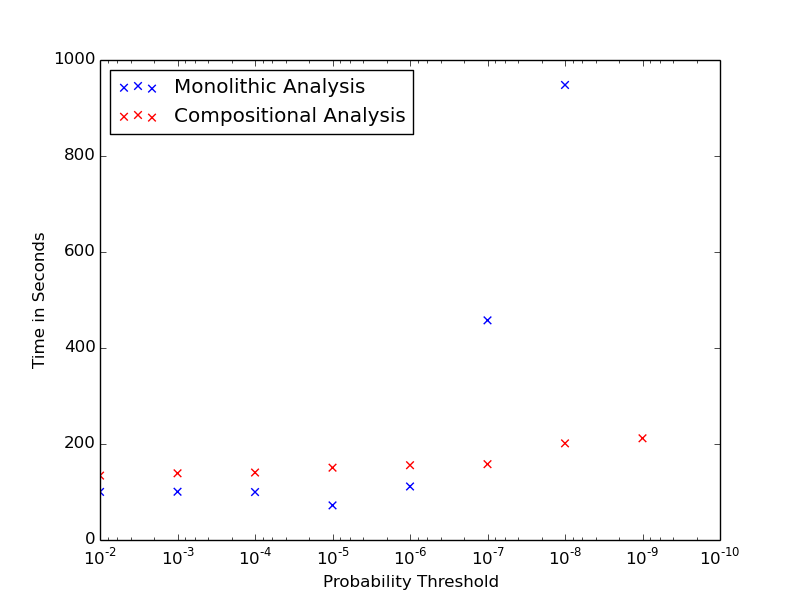
\includegraphics[width=.7\textwidth]{images/graphProbWBS_4wheel.png}
	\end{center}
	\vspace{-0.3in}
	\caption{Monolithic and Compositional Probabilistic Fault Analysis for the 4 Wheel Braking System}
	\label{fig:graphProbWBS_4wheel}
	%\vspace{-0.2in}
\end{figure}

The monolithic analysis shows that the time of analysis increases as the probabilistic threshold is lowered; by $1.0 \times 10^{-7}$, the time increase is noticeable. The reason for increased analysis time is that more faults must be considered in the analysis -- there are more allowable combinations that could fail together. Theoretically, the time of analysis would increase as the threshold decreased until all possible combinations were always considered in the analysis. At that point, the analysis time would level off. But what we find for monolithic analysis is that when setting the threshold at $1.0 \times 10^{-9}$, the verification returns unknown results after 55 minutes. The monolithic approach seems quite suitable for smaller models, but when many faults are introduced by lowering the threshold, the analysis cannot proceed.

When running the same models using a compositional probabilistic approach, we see that the time increases but not nearly as quickly. As expected, a compositional approach may provide a more feasible method of verification for large scale models. 

\paragraph{Minimal cut set analysis:} To analyze the results of the algorithms described in Chapter~\ref{chap:compFF}, we split the verification time into two parts; the first part includes only the generation of all MIVCs. This is a required step in the process. The second step is to show the additional time needed to transform those MIVCs into minimal cut sets. There are a number of parameters that can be used to show such results. The computation time may change if a probabilistic threshold is set that is very small, a max \textit{n} analysis threshold that is very large, or a model with many faults defined or numerous contracts. To adjust for these factors, we ran the analysis on the large wheel brake system model (WBS) for each of the safety properties and performed max \textit{n} analysis. The number of minimal cut sets generated per property at a given threshold is shown in Table~\ref{tab:wbs_maxN_results}.
\begin{table}[htbp]
\begin{center}
    \begin{tabular}{ | l | l | l | l | l | l |}
    \hline
    \textbf{Property} & $\bm{n = 1}$ & $\bm{n = 2}$ & $\bm{n = 3}$ & $\bm{n = 4}$ 
		& $\bm{n = 5}$    \\ \hline \hline
    0321 & 7 & 0 & 0 & 256 & 57,600   \\ \hline
    0322-R & 75 & 0 & 0 & 0 & 0  \\ \hline
    0322-L & 75 & 0 & 0 & 0 & 0  \\ \hline
    0323 & 182 & 0 & 0 & 0 & 0  \\ \hline
    0324 & 8 & 3,665 & 28,694 & 883,981 & - \\ \hline
    0325-WX & 33 & 0 & 0 &0 &0 \\ \hline
    \end{tabular}
    \caption{WBS Minimal Cut Set Results for Max \textit{n} Hypothesis}
    \label{tab:wbs_maxN_results}
    \end{center}
\end{table}

Each column of Table~\ref{tab:wbs_mincut} labeled with the value of \textit{n} gives the fault hypothesis threshold for that analysis run. For comparison with the number of minimal cut sets generated per property, we refer to Table~\ref{tab:wbs_maxN_results}\footnote{The property S18-WBS-0325-WX is symmetric for all eight wheels. For readability, we only include wheel one verification timing results in Table~\ref{tab:wbs_mincut}. Likewise for property 0322-L/R.}.
\begin{table}[htbp]
\begin{center}
    \begin{tabular}{ | l | l | l | l | l | l | l |}
    \hline
    \textbf{Property} &  MIVC Gen & $n=1$ & $n=2$ & $n=3$ & $n=4$ & $n=5$     \\ \hline \hline
    0321 & 396.417 & 5.913 & 5.468 & 5.61 & 5.636 & 11.925  \\ \hline
    0322-L  & 407.078 & 5.931 & 5.435 & 5.302 & 5.268 & 5.243 \\ \hline
    0323 & 412.926 & 6.397 & 6.452 & 6.420  & 5.309 & 5.459\\ \hline
    0324 & 446.610 & 41.334 & 41.744 & 44.062 & 69.142 & -\\ \hline
    0325-W1 & 391.137 & 5.632 & 5.388 &5.359 &5.301 & 5.236 \\ \hline
    \end{tabular}
    \caption{WBS Analysis Time in Seconds}
    \label{tab:wbs_mincut}
    \end{center}
\end{table}

The overall time of the algorithms used for minimal cut set generation is quite small compared to the nominal analysis and extended model analysis time. This is not altogether surprising; the nominal and extended analysis is contending with an infinite state model checking problem whereas the algorithms presented to generate minimal cut sets deal with set element algorithms and boolean formula manipulation. The greatest time recorded was for property S18-WBS-0324 at $n = 4$; the reason is clear when comparing this with Table~\ref{tab:wbs_maxN_results}: the total number of minimal cut sets computed for this threshold is 916,349. 
 
In summary, there are multiple ways of comparing analysis timing results and we tried to account for these by providing meaningful comparisons between some important factors. Practically, the method of using compositional verification in safety analysis is a feasible approach in both large and small models. These comparisons support the goal of the research which is to provide usable and automated safety analysis methods to analysts. 






\begin{comment}
\paragraph{Max \textit{n} analysis, compositional:} In this form of analysis, the model is verified per architectural layer from the top down. Any active faults occur {\em per layer} and any counterexamples only take that layer into account. For timing results, we compare the nominal model analysis time with the complete fault analysis time per model. The nominal analysis contains no extended fault model information in the Lustre file.  

\begin{figure}[htbp]
	%\vspace{-0.2in}
	\begin{center}
		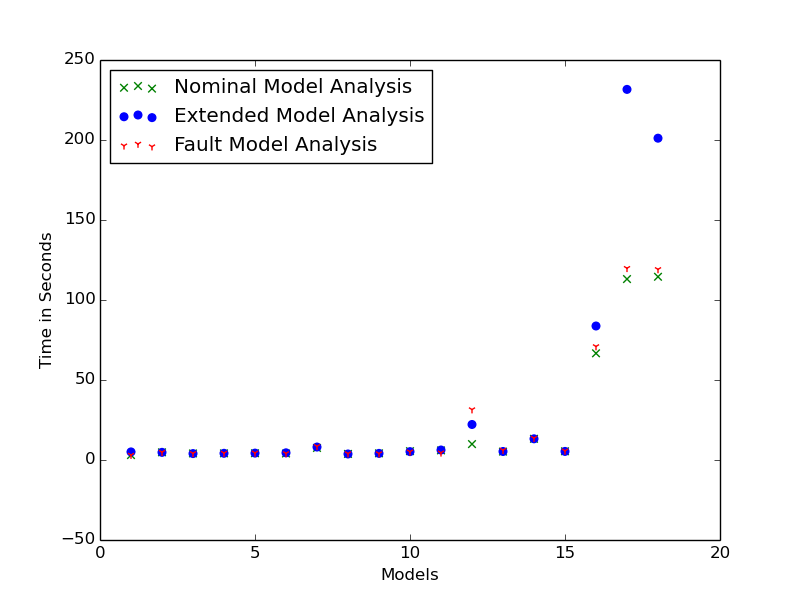
\includegraphics[width=.7\textwidth]{images/graphComp15Models.png}
	\end{center}
	\vspace{-0.3in}
	\caption{Compositional Nominal and Fault Analysis Comparison}
	\label{fig:graphComp15Models}
	%\vspace{-0.2in}
\end{figure}

As shown in Figure~\ref{fig:graphComp15Models}, the difference in fault analysis time (with max 4 fault hypothesis statement) and the nominal time is in most cases comparable. In models 14 and 15, the fault analysis time is interestingly less than the nominal. \danielle{Why is this less? What could be the reason?}

\paragraph{Max \textit{n} analysis, monolithic:} Monolithic analysis takes a flattened model and proves the safety properties given all contracts on all components. The fault hypothesis statement (max \textit{n} analysis) constrains the number of active faults; this value -- depending on the model -- may change the timing of analysis. For our purposes, we set \textit{n} constant in the analysis runs for $n = 4$. For some of the models, this is above the highest cardinality of any cut set produced, for others this is not the case. Then we compare the timing results between nominal and fault analysis for the given models. The models are numbered the same as in Figure~\ref{fig:graphComp15Models}.

\begin{figure}[htbp]
	%\vspace{-0.2in}
	\begin{center}
		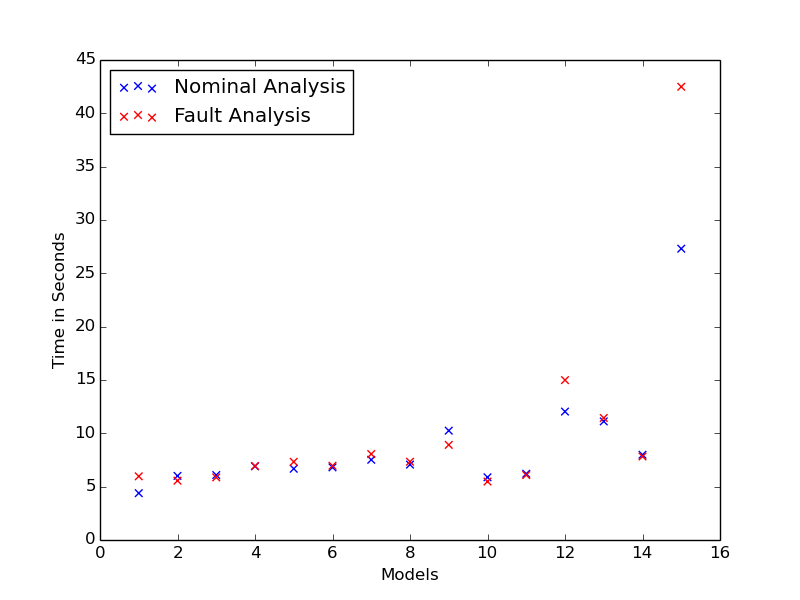
\includegraphics[width=.7\textwidth]{images/graphMono15Models.png}
	\end{center}
	\vspace{-0.3in}
	\caption{Monolithic Nominal and Fault Analysis Comparison}
	\label{fig:graphMono15Models}
	%\vspace{-0.2in}
\end{figure}

As shown in Figure~\ref{fig:graphMono15Models}, the difference in fault analysis time (with max 4 fault hypothesis statement) and the nominal time using monolithic verification is in most cases comparable. A notable exception is in model 15; in the monolithic case, the fault model verification is slower than nominal. It is the opposite for compositional. \danielle{Why? What is a possible reason for this?}

\paragraph{Max \textit{n} analysis, generation of minimal cut sets:} For the generation of minimal cut sets, the nominal model is first proved compositionally; the faults are defined on each component, constrained to false, and are flagged as MIVC elements for consideration. The results from this analysis -- the MIVCs -- are then used to generate all MCSs. The MCSs are then transformed into minimal cut sets. 

We compare the timing results using three data points: (1) the unextended nominal model analysis time, (2) the extended fault model analysis time, and (3) the additional time required to transform the MIVCs to minimal cut sets. The third data point is the difference between the total time it takes to generate minimal cut sets and the time required to generate all MIVCs from the extended fault model. For the initial run on the set of 15 models, we set the hypothesis to max 4 faults for consistency. 

\danielle{Run 15 models gen mcs.}


\begin{table}[htbp]
\begin{center}
    \begin{tabular}{ | l | l | l | l |}
    \hline
    \textbf{Property} & MIVC Gen & Min Cut Sets $n=4$     \\ \hline \hline
    1 & 2.021 & 5.073   \\ \hline
    2 & 3.310 & 0.158  \\ \hline
    3 & 1.917 & 0.043  \\ \hline
    4 & 1.899 & 0.105   \\ \hline
    5 & 2.343 & 0.052   \\ \hline
    6 & 1.759 & 0.039    \\ \hline
    7 & 7.893 & 0.108   \\ \hline
    8 & 2.448 & 1.924  \\ \hline
    9 & 5.051 & 4.808  \\ \hline
    10 & 3.965 & 0.084   \\ \hline
    11 & 4.075 & 0.140    \\ \hline
    12 & 67.791 & 0.835   \\ \hline
    13 & 5.556 & 7.155  \\ \hline
    14 & 9.607 & 0.341   \\ \hline
    15 & 12.192 & 26.009  \\ \hline
    16 & 122.403 & 11.200  \\ \hline
    17 & 495.198 & 77.443  \\ \hline
    18 & 12.192 & 26.009  \\ \hline
    \end{tabular}
    \caption{18 Models Analyses: Time in Seconds}
    \label{tab:wbs_mincut}
    \end{center}
\end{table}


\danielle{Say something about results}

For timing results on a much larger system than what is included in the 15 model set above, see Section~\ref{sec:wbs}. 

\paragraph{Probabilistic analysis, generation of minimal cut sets:} We set the probabilistic threshold (hypothesis statement) to be $1.0 \times 10^{-9}$ for all safety properties for all models and show the comparison between the nominal model analysis and the minimal cut set generation procedures. 

\danielle{Figure out how to treat this case.}

\paragraph{Probabilistic analysis, monolithic:} In this case, the constraint on the active faults is given in terms of probability. Since each fault has probability of occurrence specific to the component and the domain, it is difficult to capture all information in the results, so we set the probabilistic threshold to $1.0 \times 10^{-9}$ to allow for multiple fault activations and let the fault occurrence probability match that of the domain and component. 

Given that the various models have differing probabilistic thresholds {\em per property}, it is difficult to make meaningful comparisons between the models. In most cases, the trend is that the timing between nominal and fault analysis is close when given sufficiently high probability threshold. The time gap between the analyses widens as probability threshold decreases; the reason being that more faults must be considered in the analysis. In every case, this continues until it levels out due to the inclusion of every fault in the model being part of a minimal cut set. 
\end{comment}
